\documentclass[12pt,oneside]{paper}
\usepackage{listings}
\usepackage{lscape}

\lstset{%
  language={C},
  basicstyle={\small},%
  identifierstyle={\small},%
  commentstyle={\small\itshape},%
  keywordstyle={\small\bfseries},%
  ndkeywordstyle={\small},%
  stringstyle={\small\ttfamily},
  frame={tb},
  breaklines=true,
  columns=[l]{fullflexible},%
  numbers=left,%
  xrightmargin=0zw,%
  xleftmargin=3zw,%
  numberstyle={\scriptsize},%
  stepnumber=1,
  numbersep=1zw,%
  lineskip=-0.5ex%
}

% タイトル
\title{データログシステムの研究}
\author{藤井岳寛}

\begin{document}
% 行間
\setlength{\baselineskip}{9truemm}

%文字間
\kanjiskip=.53zw plus 3pt minus 3pt
\xkanjiskip=.53zw plus 3pt minus 3pt

% 目次
\tableofcontents
%\newpage

% 本文

\chapter{序論}
\section{研究の背景}
本研究室では毎年高専ロボコンに参加していて,去年まで3年連続で全国大会に出場している.
今年は地区大会を優勝し,全国大会に出場することを目標とした.
試合に勝つための作戦を考え,その作戦を実行できるロボットを設計・製作した.
しかし,地区大会初戦で原因不明のマシントラブルに見舞われ敗退した.
原因不明というのは,試合後は正常に動作し現象が再現されないこと.
そしてロボットのデータログを記録していなかったため,状況を再現して検証が行えないため.
学校での動作試験でも原因不明の不具合に幾度が見舞われたが,
現象を再現できず,対応に遅れ結果的にロボット完成が遅れた.
これらのことから,ロボットのデータログを記録していれば多くの不具合を修正でき,
上位入賞できたのではないかと考える.\\


\begin{figure}[H]
 \begin{center}
  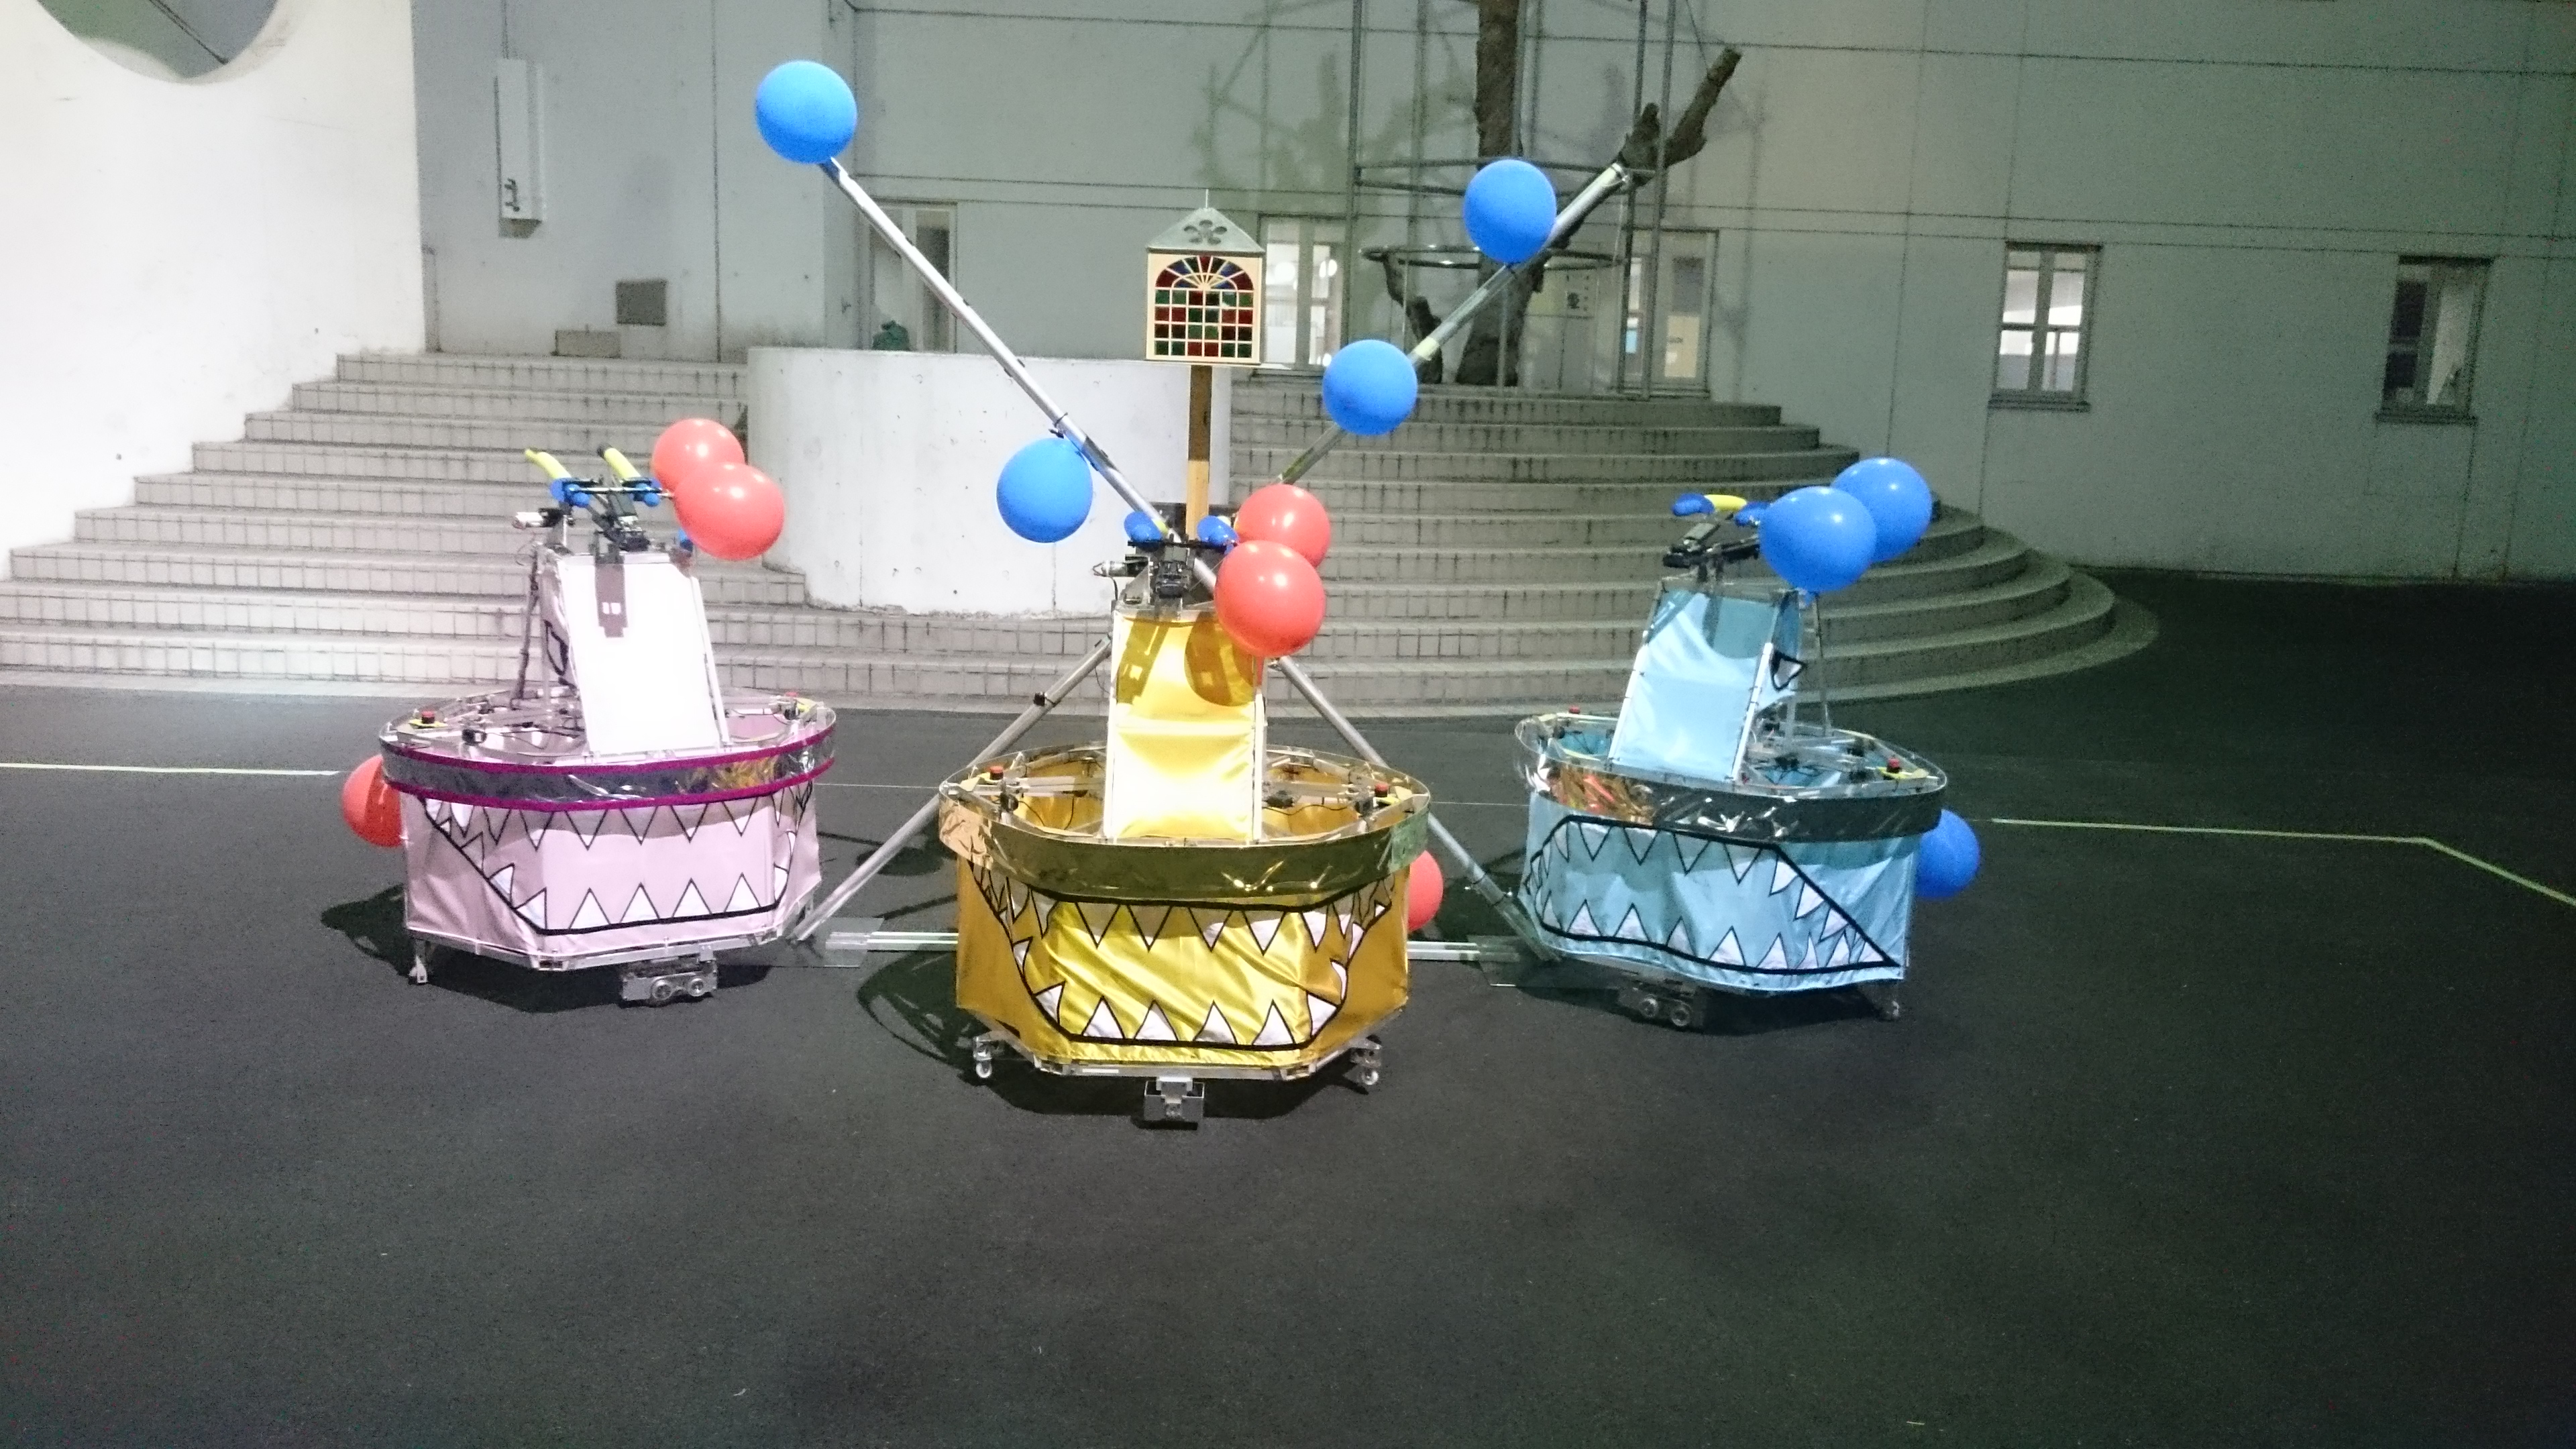
\includegraphics[width=150mm]{robot1.jpg}
 \end{center}
 \caption{今年度制作したロボット}
 \label{fig:robot1}
\end{figure}


\section{高専ロボコンについて}
アイデア対決・全国高等専門学校ロボットコンテストの略称であり,NHKが主催するロボットコンテストの1つである.
高等専門学生の甲子園といわれていて,ロボコンに憧れて高専へ入学した人も多いだろう.
各校A,Bの2チーム参加でき,地区大会の優勝チームと推薦チームが全国大会へ出場できる.
本研究室では2014年から2016年まで連続で全国大会に出場していた.
本研究室で過去に制作されたロボットたちを下図に示す.\\


\begin{figure}[H]
 \begin{center}
  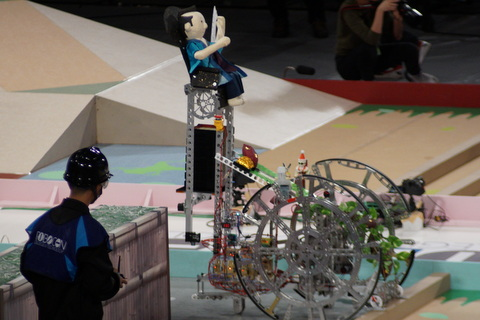
\includegraphics[width=70mm]{pote.jpg}
 \end{center}
 \caption{ポテ☆ゴロー}
 \label{fig:pote}
\end{figure}


\begin{figure}[H]
 \begin{center}
  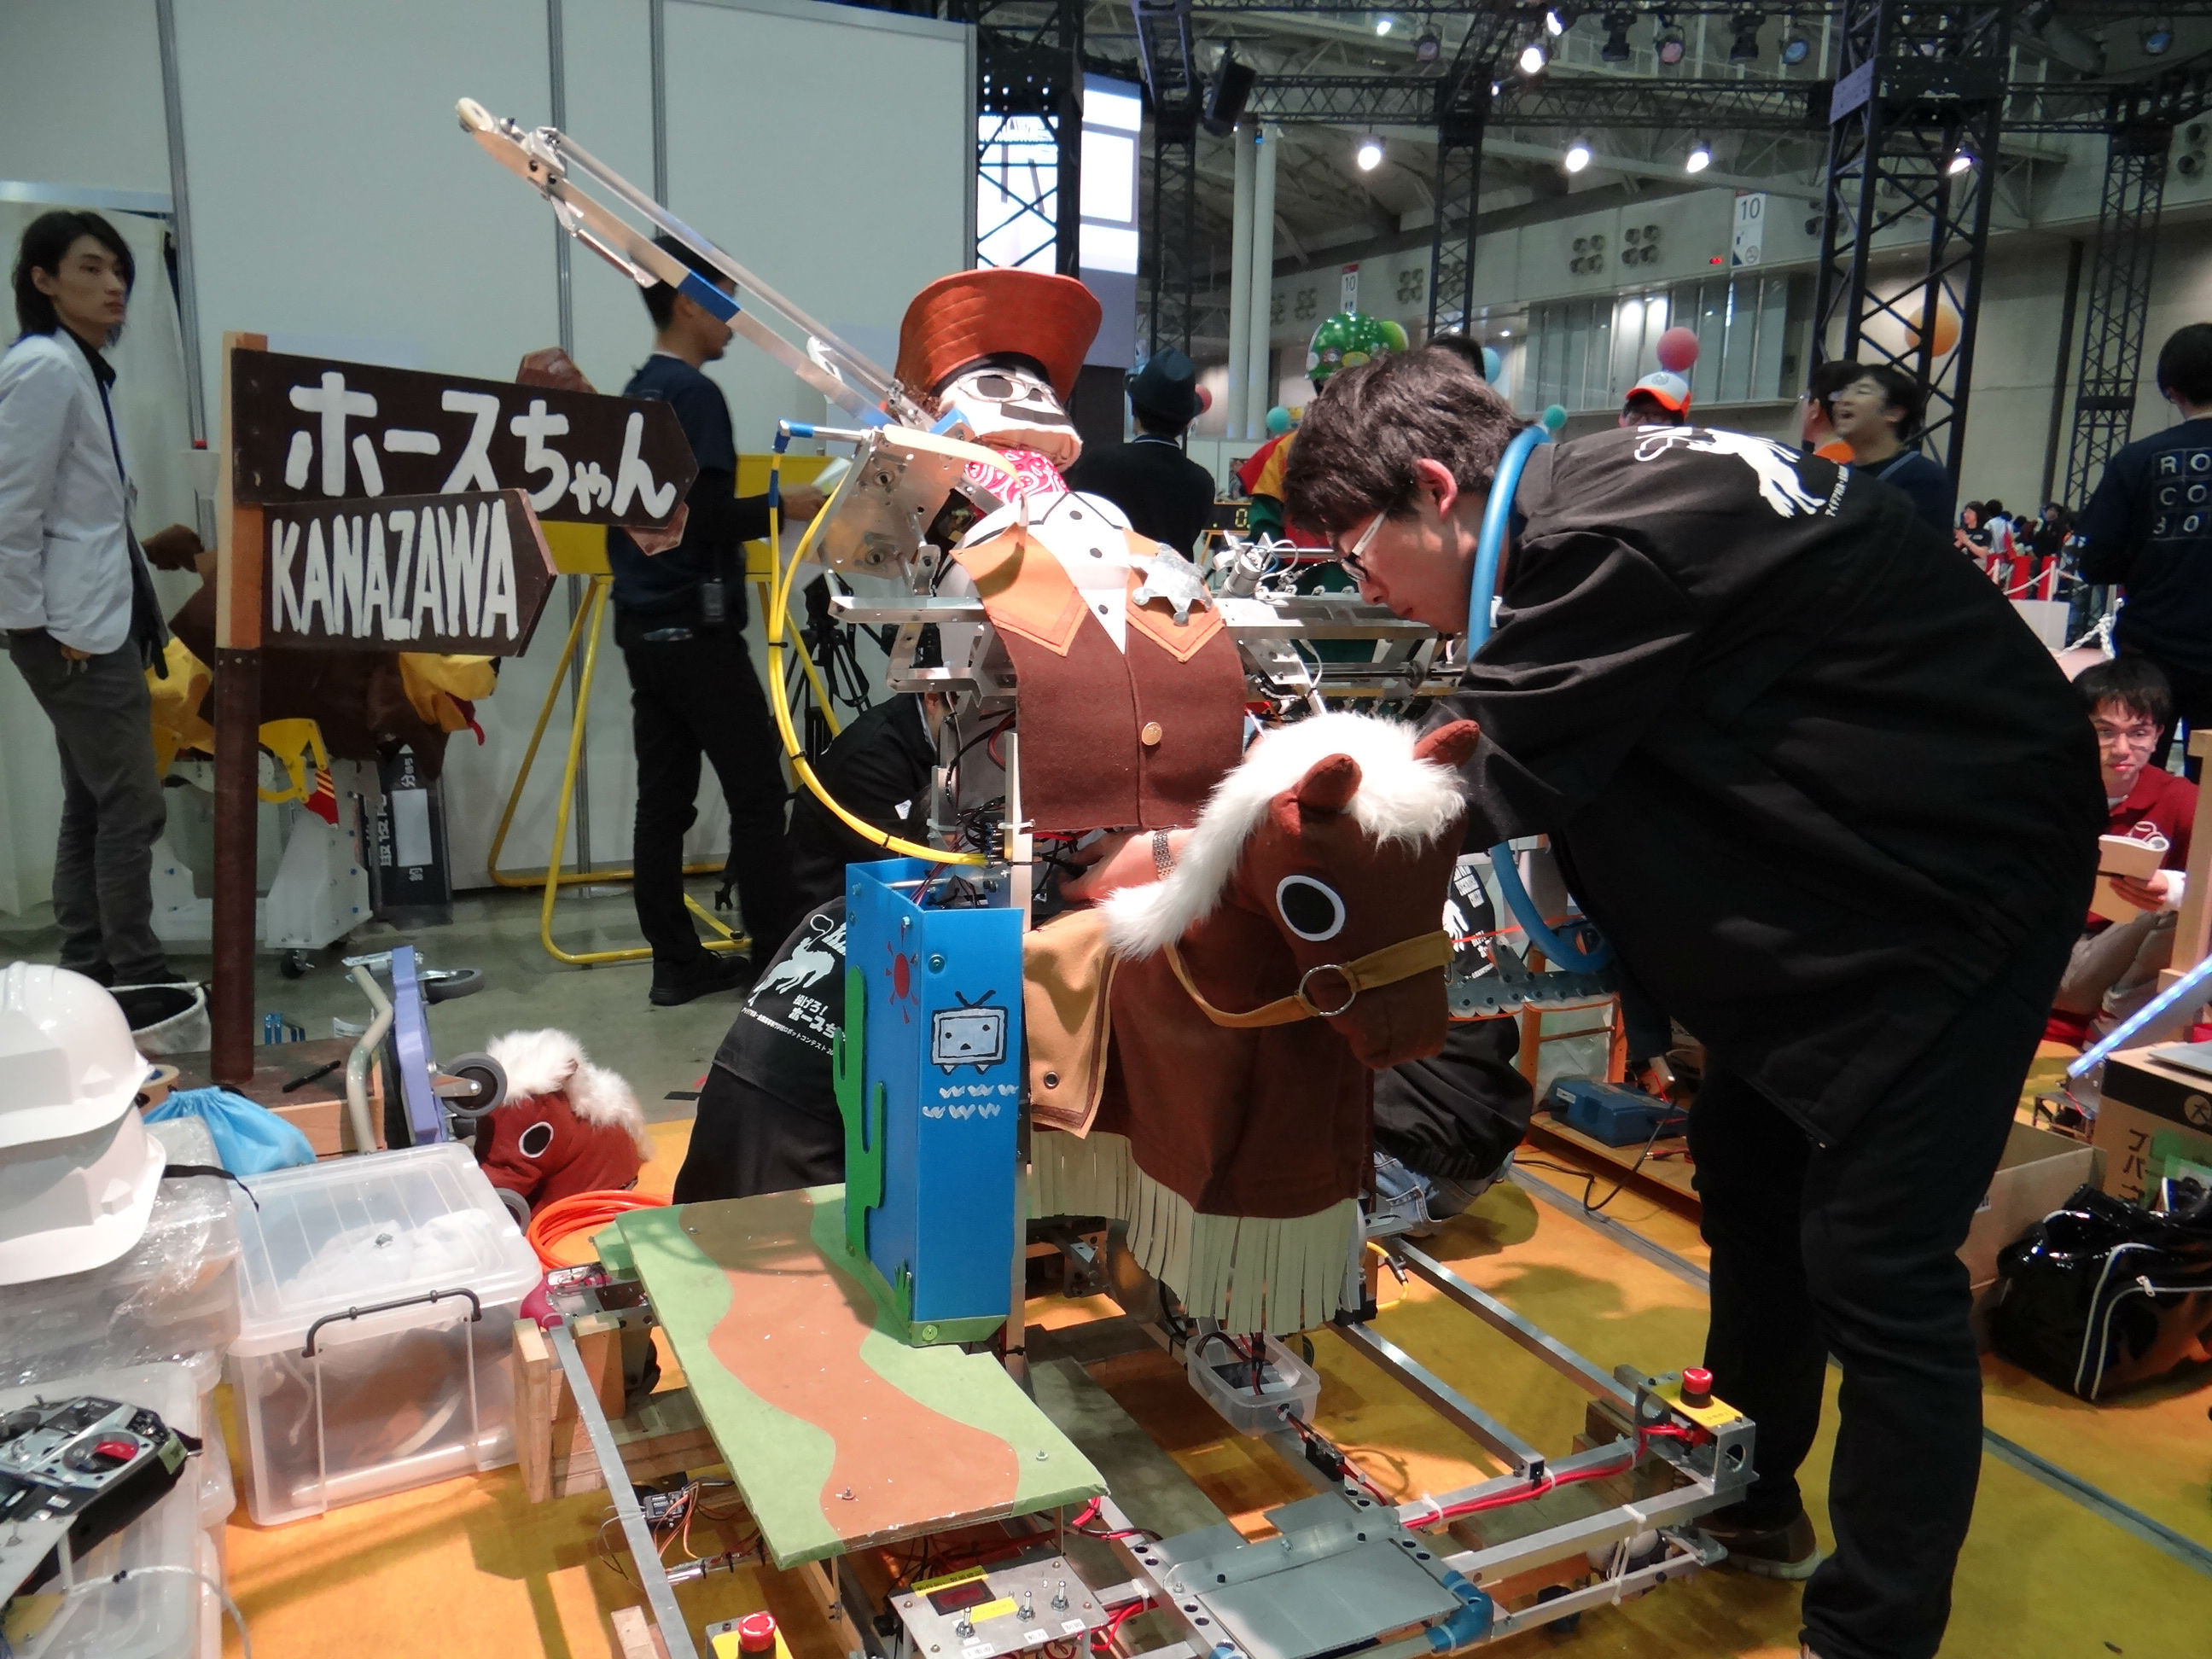
\includegraphics[width=120mm]{horsechan.jpg}
 \end{center}
 \caption{投げろホースちゃん}
 \label{fig:horse}
\end{figure}


\begin{figure}[H]
 \begin{center}
  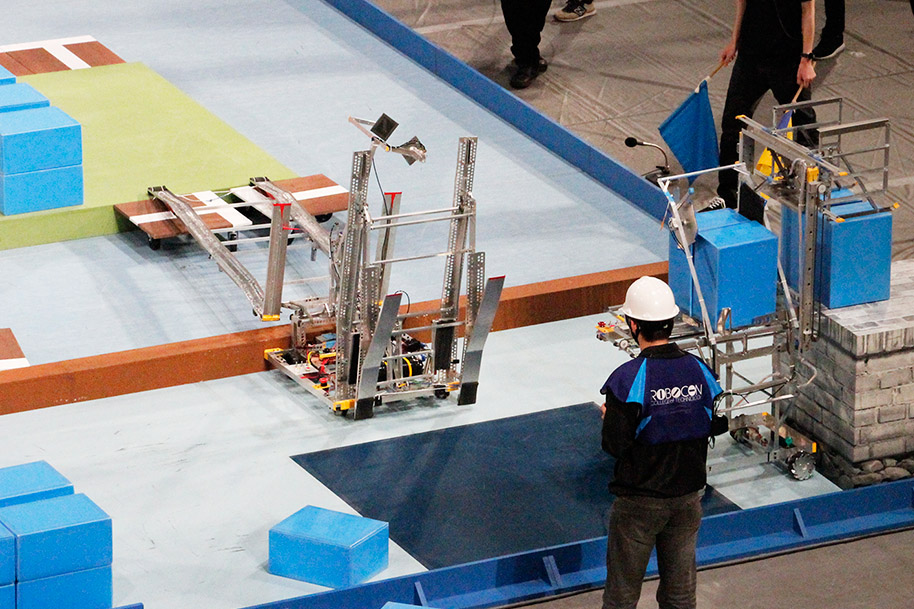
\includegraphics[width=120mm]{kotutumi.jpg}
 \end{center}
 \caption{鼓積}
 \label{fig:tutumi}
\end{figure}


\section{研究の目的}
今まではロボットの制御システムから設計を始め,マイコンの選定などを行ってきた.
しかし,毎回そこから始めるのは大変で,時間がかかるため効率的ではない.
そこで,本研究室のロボコン用標準制御システムを考案し,
それをベースとして制御システムの開発をすることにより開発にかかる時間を短縮する.
加えて,標準制御システムのデータログシステムを開発することによりトラブルシューティングの効率化を図る.
標準制御システムのマニュアルを作成することで,プログラムが苦手な機械科学生でも制御システムの開発を行えるようにし,
来年度以降のロボコン活動を支援する.


\section{論文の構成}
この論文では以下のように構成されている.
1章では,研究目的や高専ロボコンの説明,今年度の敗因について考察したものである.


2章では,ロボコンの標準制御システム考案とロボコンShieldについて述べる.


3章では,本研究で作成したログシステムについて述べる.


4章では,本研究のまとめを述べる.


\chapter{標準制御システムのあるべき姿}.\\

\section{要求スペックの検討}
今回はArduinoMegaをメインとして使用した制御システムを構成したが,
ロボコン用ロボットに必要なマイコンはどのくらいのスペックが要求されるのか
今年度使用したマイコンのスペック表\ref{spec1}を元に検討した結果表\ref{spec2}のようになった.


\begin{table}[h]
 \begin{center}
  \label{spec1}
  \caption{今年度のマイコンスペックと使用用途}
  \scalebox{0.65}{
  \begin{tabular}[htbp]{|c|c|p{9cm}|}
  \hline
  項目 & 数 & 使用用途,詳細 \\
  \hline
  デジタルIO & 54 & ソレノイド5つの制御,実装予定だった近接センサ2つ \\
  \hline
  アナログIO & 16 & 使用しなかった \\
  \hline
  pwmピン & 15 & 今回はServoShieldを使用したため使用しなかった \\
  \hline
  シリアルポート & 4 & タイヤ1つにつき1つで最大3つ使用した \\
  \hline
  USBホスト & 1 & USBHostShieldで追加してコントローラとの通信に使用した \\
  \hline
  \end{tabular}
  }
 \end{center}
\end{table}


\begin{table}[!h]
 \begin{center}
  \label{spec2}
  \caption{要求スペック}
  \scalebox{0.65}{
  \begin{tabular}[htbp]{|c|c|p{9cm}|}
  \hline
  項目 & 数 & 理由 \\
  \hline
  デジタルIO & 16 & ソレノイドやLEDを使うのに多く必要 \\
  \hline
  アナログIO & 4 & アナログデータが必要なアクチュエータやセンサをする場合に必要 \\
  \hline
  pwmピン & 16 & サーボモータの制御に使うため \\
  \hline
  シリアルポート & 4 & 今年度は3輪オムニの制御に3つ使用したが,4輪メカナムや4輪オムニなどを使用するには4つ必要である \\
  \hline
  SDカードソケット & 1 & データログを記録するためにSDカード使う \\
  \hline
  USBホスト & 1 & Bluetoothドングルを使いBluetooth通信するため \\
  \hline
  \end{tabular}
  }
 \end{center}
\end{table}


\section{Arduinoの性能比較}
今回の高専ロボコンではライブラリが豊富であり比較的開発が簡単であるArduinoシリーズの中で
Serialポートが3つあるArdinoMegaを使用したが,Arduinoの性能を調べ比較してみる.
各Arduinoの性能をまとめた表\ref{arduinospec}を下に示す.


\begin{table}[h]
 \begin{center}
  \label{arduinospec}
  \caption{Arduinoスペック一覧}
  \scalebox{0.7}{
  \begin{tabular}[htbp]{|c|c|c|c|c|c|}
  \hline
  名前 & ArduinoUNO & Arduino101 & ArduinoPRO & ArduinoProMini & ArduinoMega2560  \\
  \hline
  大きさ & 68.6$\times$53.4mm & 68.6$\times$53.4mm & 43$\times$18mm & 101.52$\times$53.3mm & 56$\times$25mm  \\
  \hline
  重さ & 25g & & 9g & & 37g  \\
  \hline
  価格 & 3200 & 4980 & 1868 & 1243 & 5830 \\ 
  \hline
  マイコン & ATmega328P & InrelCurie & ATmega328 & ATmega328 & ATmega2560   \\
  \hline
  動作電圧 & 5V & 3.3V & 3.3or5V & 5V & 3.3or5V  \\
  \hline
  電源電圧 & 7-20V & 7-20V & 3.35-12V & 3.35-12V & 6-20V \\ 
  \hline
  デジタルIO & 14 & 14 & 14  & 14 & 54  \\
  \hline
  アナログIO & 6 & 6 & 6 & 8 & 16  \\
  \hline
  pwmピン & 6 & 4 & 6 & 6 & 15  \\
  \hline
  シリアルポート & 1 & 1 & 1 & 1 & 4  \\
  \hline
  フラッシュメモリ & 32kB & 196kB & 32kB & 32kB & 256kB  \\
  \hline
  SRAM & 2kB & 24kB & 2kB & 2kB & 8kB  \\
  \hline
  EEPROM & 1kB & & 1kB & 1kB & 4kB  \\
  \hline
  クロック & 16MHz & 32MHz & 8or16MHz & 8or16MHz & 16MHz  \\
  \hline
  \hline
  名前 & ArduinoYUN & ArduinoDUE & ArduinoMegaADK & ArduinoEthrnet & ArduinoLeonardo  \\
  \hline
  大きさ & 101.52$\times$53.3mm & 101.52$\times$53.3mm & 68.6$\times$53.3mm & 68.6$\times$53.4mm & 28$\times$65mm \\
  \hline
  重さ & 36g & 36g & 28g & 20g & 9g \\
  \hline
  価格 & 9990 & 6264 & 8208 & 7676 & 3132  \\
  \hline
  マイコン & ATmega32U4 & AT91SAM3X8E & ATmega2560 & ATmega328 & ATmega32U4 \\
  \hline
  動作電圧 & 5V & 3.3V & 5V & 5V & 5V \\
  \hline
  電源電圧 & 5V & 6-16V & 6-20V & 6-20V & 7-12V \\
  \hline 
  デジタルIO & 20 & 54 & 54 & 14 & 20 \\
  \hline 
  アナログIO & 12 & 12 & 16 & 6 & 12 \\
  \hline
  pwmピン & 7 & 12 & 15 & 5 & 7  \\
  \hline
  シリアルポート & 1 & 4 & 4 & 1 & 1  \\
  \hline 
  フラッシュメモリ & 32kB & 256kB & 256kB & 32kB & 32kB  \\
  \hline
  SRAM & 2.5kB & 96kB & 8kB & 2kB & 2.5kB  \\
  \hline
  EEPROM & 1kB  & 4kB & 1kB & 1kB & 1kB \\
  \hline
  16MHz & 84MHz & 16MHz & 16MHz & 16MHz & 16MHz \\
  \hline
  \end{tabular}
  }
 \end{center}
\end{table}


\section{GRシリーズ}
Arduinoシリーズでは各種IOに関しては十分なものもあるが,
USBhostやSDカードスロットがなく機能を追加するにはいくつもShieldという基板を重ねなければならない.
そこで,USBhostやSDカードスロットが既存で備わっている
GRシリーズのスペックをまとめ検討する.
GRシリーズの性能をまとめた表\ref{GR}を下に示す.
\begin{table}[h]
 \begin{center}
  \label{GR}
  \caption{GRスペック一覧}
  \scalebox{1}{
  \begin{tabular}[htbp]{|c|c|c|c|}
  \hline
  名前 & GR-SAKURA & GR-KAEDE & GR-PEACH \\
  \hline
  大きさ & 53.34$\times$65.58mm & 53.84$\times$91.83mm & 53.84$\times$67.58mm \\
  \hline
  価格 & 4640 & 7500 & 9690 \\
  \hline
  マイコン & RX63N & RX64N & RZ/A1H \\
  \hline
  動作電圧 & 3.3V & 3.3V & 3.3V \\
  \hline
  電源電圧 & 5V & 5V & 5V \\
  \hline
  デジタルIO & 55 & 29 & 52 \\
  \hline
  アナログIO & 16 & 12 & 6 \\
  \hline
  pwmピン & 9 & 9 & 6 \\
  \hline
  シリアルポート & 6 & 4 & 7 \\
  \hline
  フラッシュメモリ & 32kB & 64kB & 8MB \\
  \hline
  SRAM & 128kB & 552kB & 10MB \\
  \hline
  EEPROM & 1MB & 4MB & 8MB \\
  \hline
  クロック & 96MHz & 96MHz & 400MHz \\
  \hline
  \end{tabular}
  }
 \end{center}
\end{table}

\section{GR-SAKURA}
GR-SAKURA FULLをメインマイコンに選定した.
GR-SAKURAを図\ref{fig:sakura}に示す.\\
\begin{figure}[H]
 \begin{center}
  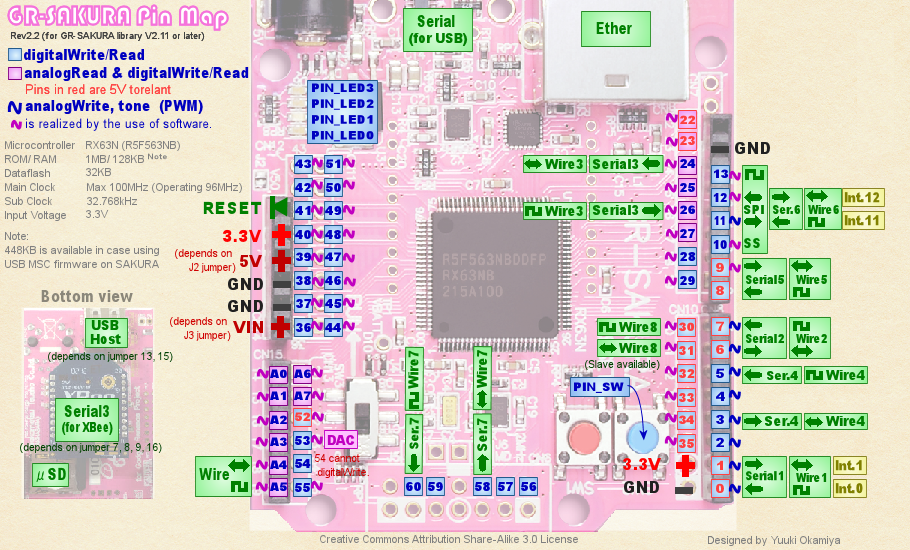
\includegraphics[width=130mm]{sakura.png}
 \end{center}
 \caption{GR-SAKURA}
 \label{fig:sakura}
\end{figure}
図\ref{fig:sakura}からわかるようにGR-SAKURAは豊富なIOに加えて
LANコネクタ,USBホストコネクタ,SDMMCカードソケットを備えている.\\


\section{今年度の構成}
ShieldとはArduinoマイコンに機能を追加するための基板であり,
モータ制御するためのものやLCDが付いたものなど多くの種類が存在する.
それらをArduinoに重ねることにより多くの機能をArduinoに持たせることができる.
今年度はArduinoMegaにコントローラーとBluetooth通信するためのUSBhostShieldと
サーボモータを制御するためのAdafruit16-ChannelServoShieldを載せ,
さらに各種IOを使いやすくするための自作Shieldも搭載した.
今年度のロボット制御基板を図\ref{fig:kiban}に示す.


\begin{figure}[H]
 \begin{center}
  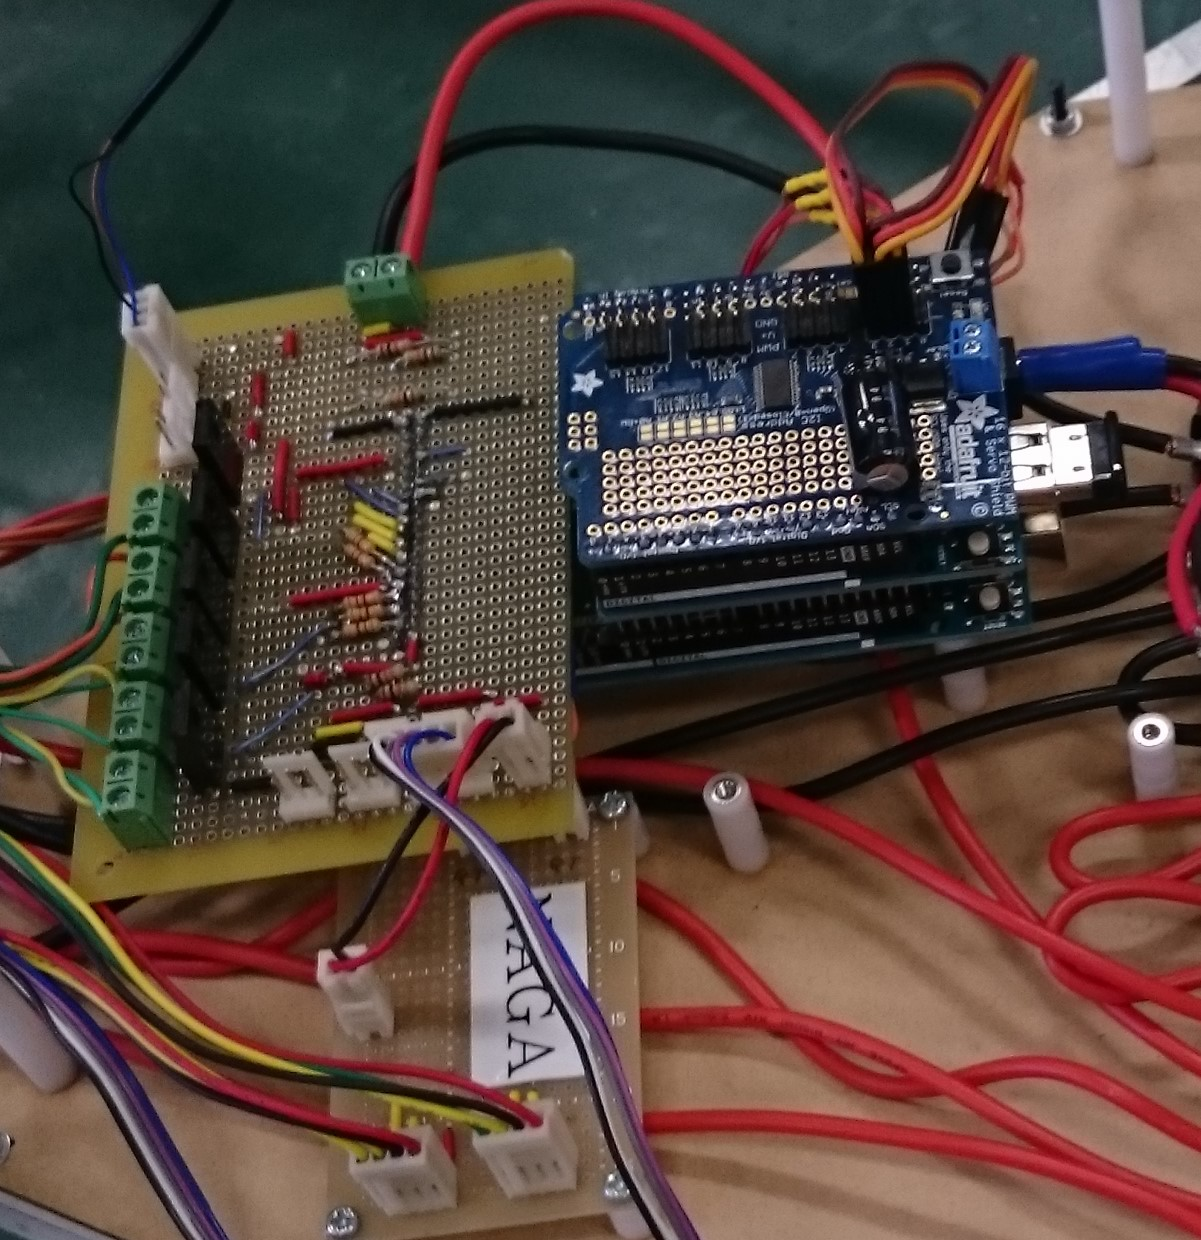
\includegraphics[width=150mm]{kiban.jpg}
 \end{center}
 \caption{制御基板}
 \label{fig:kiban}
\end{figure}

\section{ロボコンshield}
GR-SAKURAはUSBhostやSDカードスロットが既存であるため,
シリアル通信の規格をRS485に変換するトランシーバと各種IOを外側に出し接続しやすくするものを作成する.
ロボコンシールドを設計するにあたり,GR-SAKURAの詳細な寸法を調査した.
GR-SAKURAの詳細寸法を図\ref{fig:sunpo}に示し,ロボコンシールドの回路図を図\ref{fig:kairo1}に示す.\\

\begin{figure}[H]
 \begin{center}
  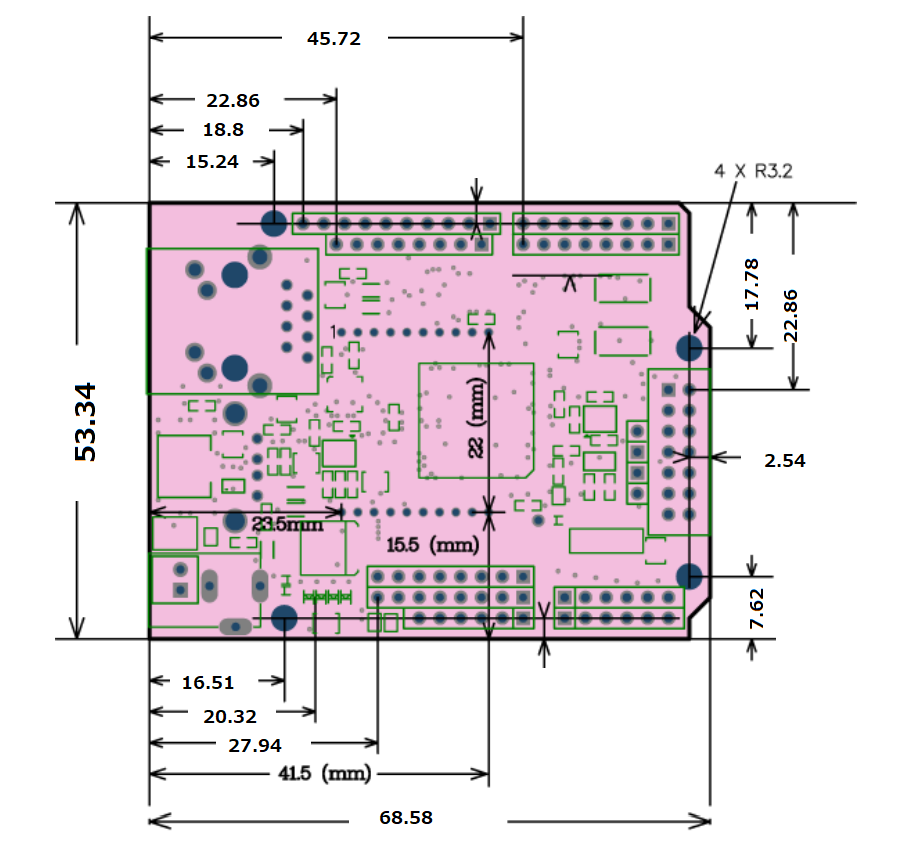
\includegraphics[width=150mm]{gr.png}
 \end{center}
 \caption{GR-SAKURA詳細寸法}
 \label{fig:sunpo}
\end{figure}

\begin{figure}[H]
 \begin{center}
  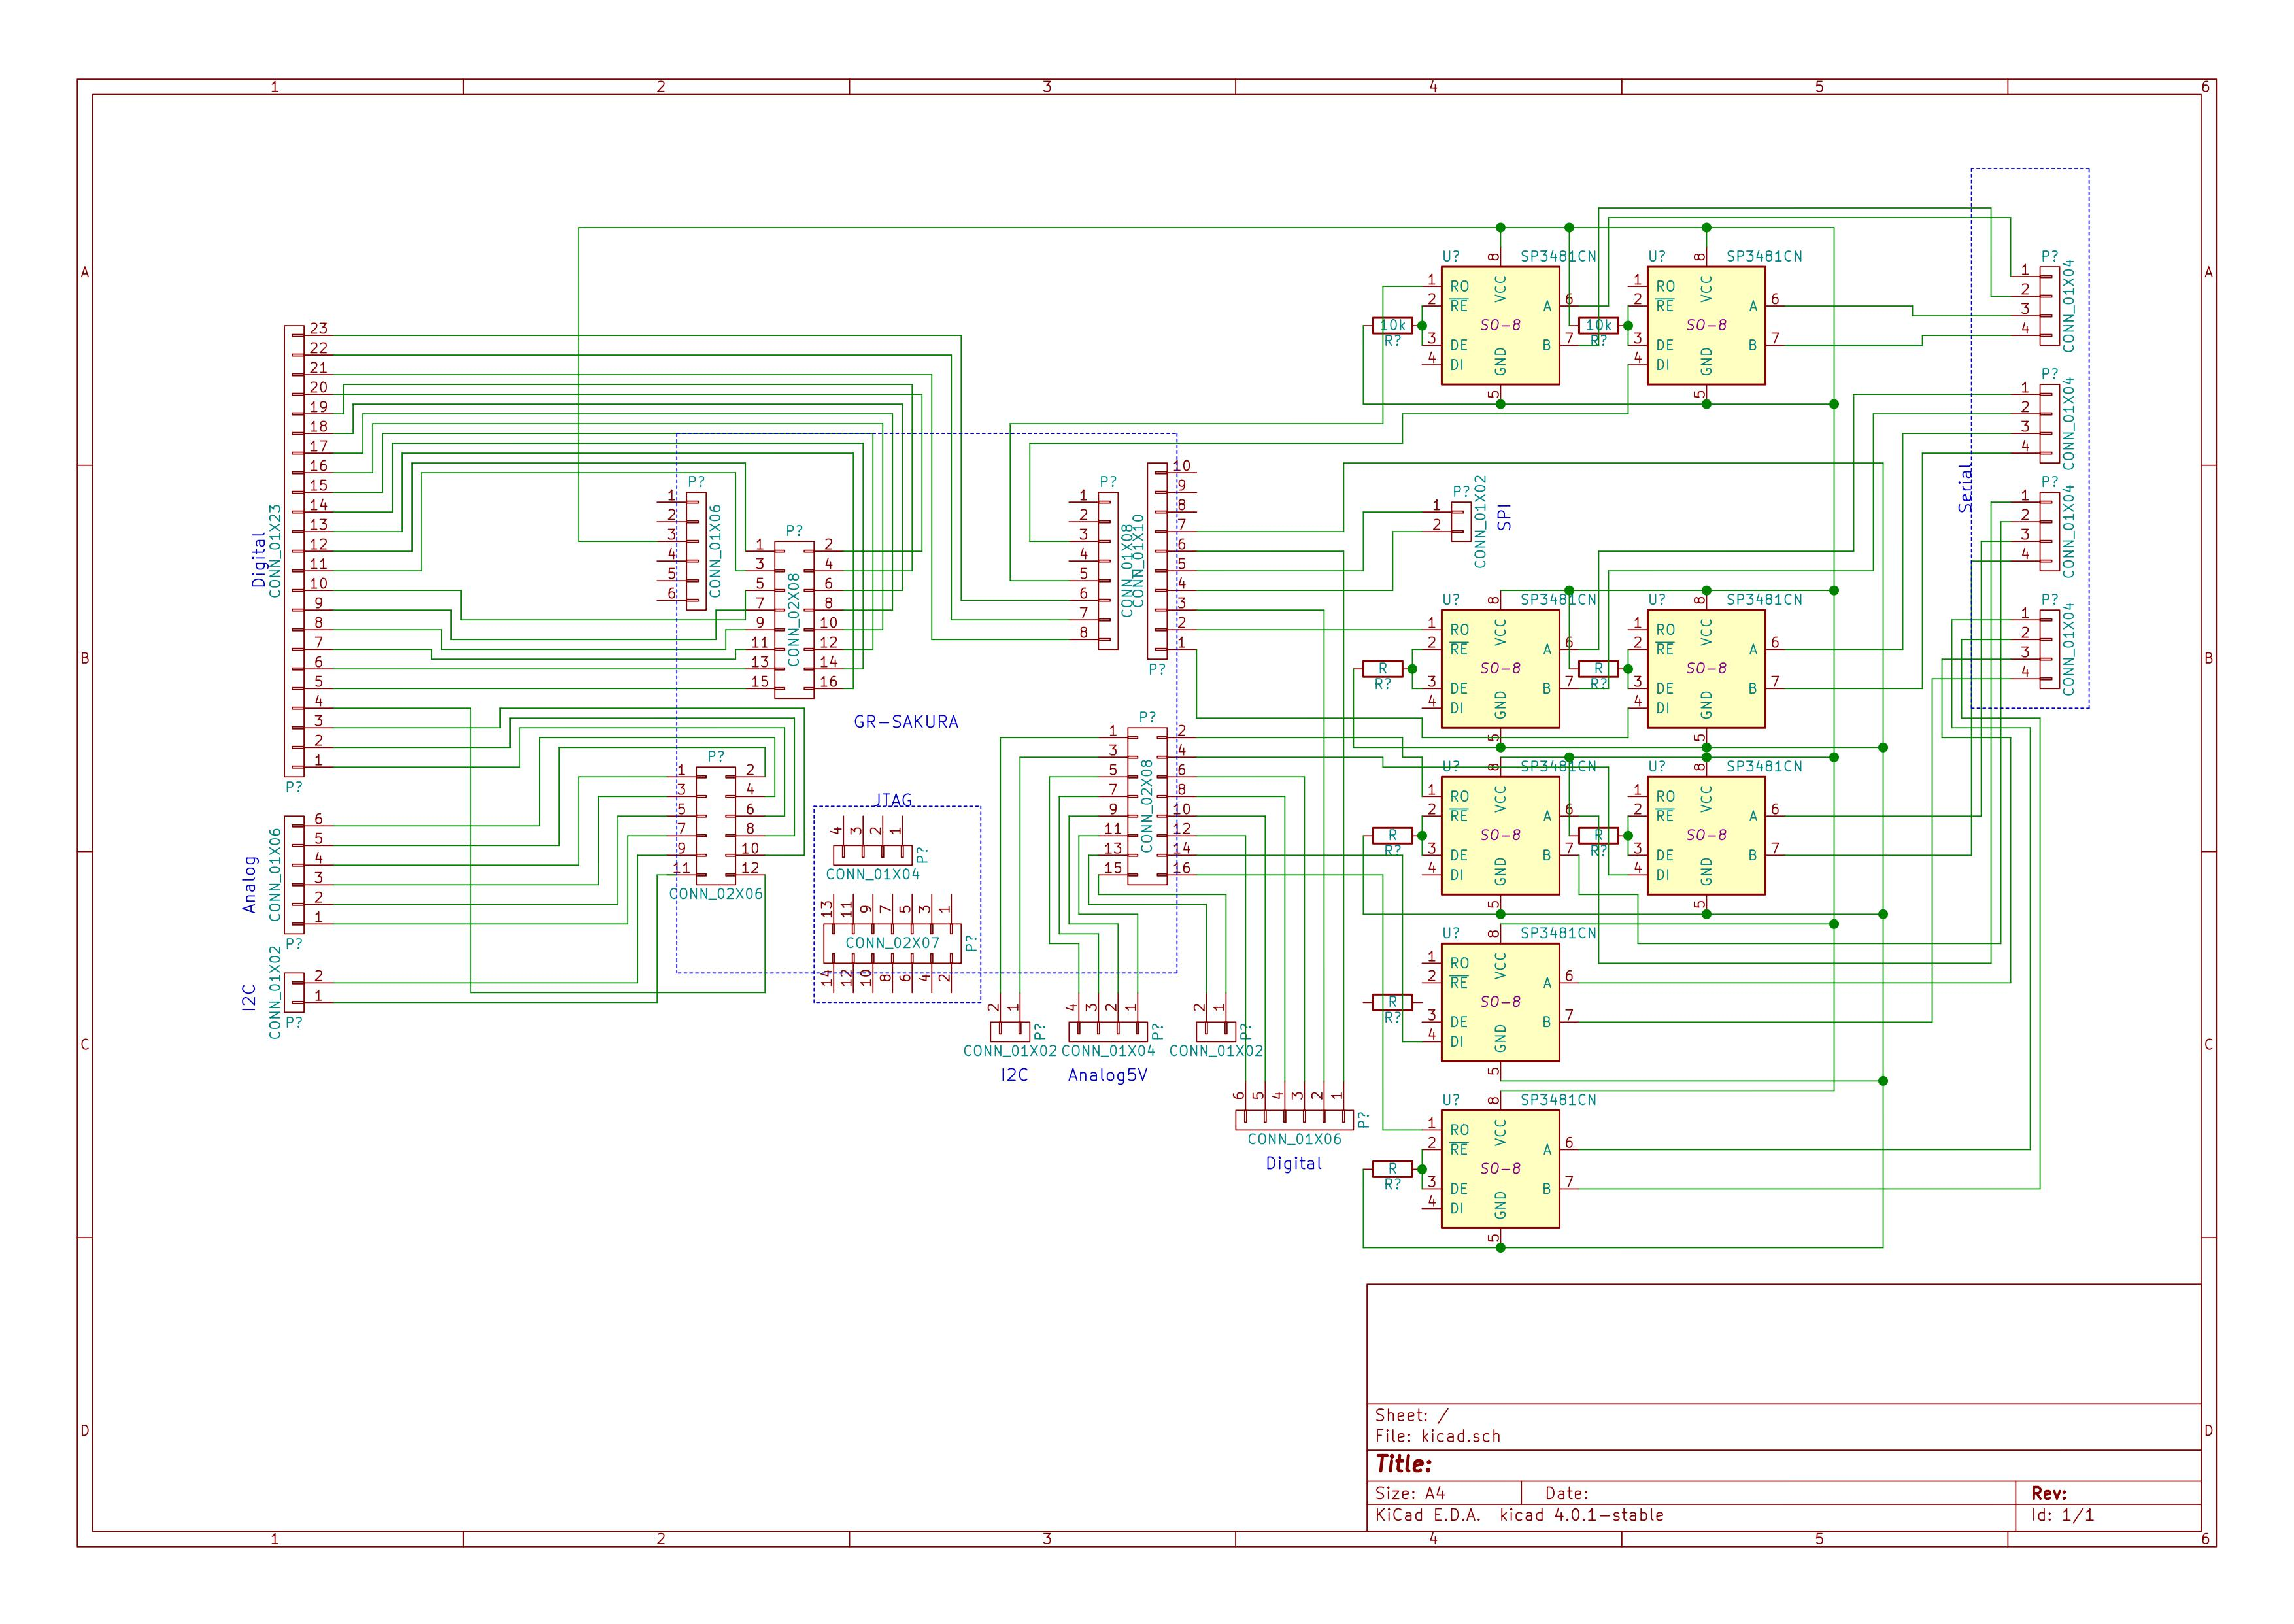
\includegraphics[width=150mm]{0001.jpg}
 \end{center}
 \caption{シールド回路図}
 \label{fig:kairo1}
\end{figure}


GR-SAKURAはSerial通信に使用できるポートが複数あるが,SPI通信などと兼ねているものがある.
そのため使用すると予想される最大数の4つをSerial通信に使用できるようにした.
また,今年度のSerial通信の規格はRS232Cを使用してノイズに悩まされたため,
ノイズ対策としてRS485に変換するトランシーバを搭載した.
RS-232C・RS-422A・RS-485は,EIA(Electronic Industries Association:米国電子工業会)の通信規格である.
中でもRS-232Cは,通信規格の中でも用途を問わず多く普及し,パソコンにも標準で搭載されおり,モデムやマウスの接続によく利用されている.
センサやアクチュエータの中にも,これらのインターフェイスを持ち,通信により制御可能なものもが多く存在する.
RS485は差動信号を採用している.2線間の電圧の違いによってどんなデータを伝送するか表現している.
シリアル通信の規格を次に示す.


\subsection{RS-232C}
RS-232Cでは,1本の信号線でデータを伝送するシングルエンド伝送を用いており,データを伝送するとき信号線の電圧が-5~-15Vのとき「1」となり,
電圧が+5~+15Vのとき「0」となる.電圧レベルで伝送するためノイズに弱く,規格ではケーブルの最大長は15mとなっている.
常に外部から電源を供給しているデスクトップパソコンでは高い出力電圧を得られますが,バッテリ等の低い電源で動作するノートパソコンの場合,
出力電圧も低くなります.ノートパソコンの中にはRS-232Cのポートが搭載されていても使用しない設定になっているものもある.
この場合,RS-232Cポートを使用するよう設定を行う必要がある.

\subsection{RS-422A}
ケーブルには2本の電線をより合わせて対にしたツイストペアケーブルが用いられている.2本の電線をより合わせることで,
電流が流れるときに生じる磁気を打ち消すような仕組みになっている.その中でシールドしているものをSTP(Shielded Twisted Pair cable),
していないものをUTP(Unshielded Twisted Pair cable)という. コネクタの形状は規格化されていないが,
実際に使用されるものではD-SUB9PやD-SUB25Pが多く,ミニDIN8Pや端子台も使われる.

RS-422では2本の信号線でデータを伝送する差動伝送(ディファレンシャル)を用いており,
「+」と「-」の2本の信号線でデータを伝送し +信号線の電圧が -信号線の電圧より高い場合を「1」,低い場合を「0」と判断する.
このように信号線2本の電位差で信号を判断しているため,電線延長による電圧の減衰は「+」と「-」の両方で起こり,
「+」と「-」の電位差には影響が少なくなる.0.3Vの電位差で信号と認識するため,比較的ノイズに強く長距離延長が可能となることから,
工場のようなノイズが多い環境での使用に適している.規格ではケーブルの最大長は1.2kmとなっている.

\subsection{RS-485}
RS-422の上位互換である.
RS-422が1:nに対し,RS-485はn:mの接続に対応しており,1対の信号線上に最大32台まで接続できるマルチドロップ方式になっている. 
複数の機器を接続する場合,回路の終端で信号が反射し,信号波形が乱れてしまうことがある.
このような現象が繰り返し行われていると通信速度を上げることができなかったり,正常なデータ伝送ができなくなることがある.
そこでRS-485回線には信号線の終端に信号線が持つインピーダンスと等しい抵抗(終端抵抗)を入れることで伝送中の反射を抑え,
信号波形の乱れを少なくすることができる. コネクタの形状は規格化されていないが,実際に使用されるものではRJ-45やD-SUB9P,
端子台等がある.その他の仕様はRS-422に準拠する.

\begin{table}[h]
 \begin{center}
  \label{Serial}
  \caption{Serial通信一覧}
  \scalebox{1}{
  \begin{tabular}[htbp]{|c|p{3cm}|p{3cm}|p{3cm}|}
  \hline
  パラメータ & RS232C & RS422A & RS485 \\
  \hline
  伝送モード & シンプレックス & \shortstack{マルチポイント \\ シンプレックス} & \shortstack{マルチポイント \\ マルチプレックス} \\
  \hline
  最大接続台数 & \shortstack{1ドライバ \\ 1レシーバ} & \shortstack{1ドライバ \\ 10レシーバ} & \shortstack{32ドライバ \\ 32レシーバ} \\
  \hline
  最大伝送速度 & 20kbps & 10Mbps & 10Mbps \\
  \hline
  最大ケーブル長 & 15m & 1200m & 1200m \\
  \hline
  動作モード & シングルエンド(非平衡型)& ディファレンシャル(平衡型)& ディファレンシャル(平衡型)\\
  \hline
  特徴 & \shortstack{短距離 \\ 全2重 \\ 1:1の接続} & \shortstack{長距離 \\ 全2重 半2 \\ 1:Nの接続} & \shortstack{長距離 \\ 全2重 半2重 \\ N:Mの接続} \\
  \hline
  \end{tabular}
  }
 \end{center}
\end{table}

\chapter{ログシステムの開発}
\section{ログシステムの要求項目}
ログシステムに必要な項目を挙げる.
\begin{enumerate}
 \item 指定した値の記録
 \item タイムスタンプ
\end{enumerate}
1)指定した値の記録はログシステムの主となる部分である.
製作したロボットの電圧や制御指令値など,様々な値を記録することによりトラブルが発生した時に原因を明らかにする手助けとなる.
しかし,ログとして記録する値が変更されたり増えるたびにprint文などのプログラムの中身を書き換えるのは不便である.
そこで必要な値のリストをユーザーが用意し,そのリストを読みリストで指定された値を1レコードとして記録する.


2)タイムスタンプはある出来事が発生した時間を示す文字列のことである.
ただただ値を記録していったのではただの数字の羅列になり,どこで何が起きたのかわからない.
そこで1レコードごとにタイムスタンプをつけることによりその値がいつのものなのか明らかにする.

\section{ログシステムのフローチャート}
プログラムのフローチャートを図\ref{fig:flow}に示す.
\begin{figure}[H]
 \begin{center}
  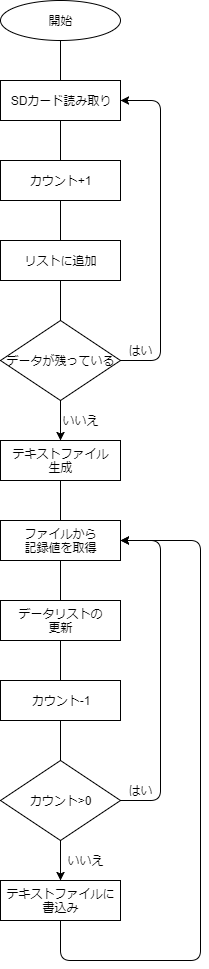
\includegraphics[width=30mm]{flow.png}
 \end{center}
 \caption{フローチャート}
 \label{fig:flow}
\end{figure}

\section{ログシステムのヘッダファイル}
ヘッダファイルはファイル読み取り時,作成されたデータの記号リストの記号にデータの値を代入するものである.
データのリストを1レコードとし,タイムスタンプを最後に加えてテキストファイルに書き込みする.
その後,リストのデータの値を更新し書込みを繰り返す仕様になっている.
ヘッダファイルをListing\ref{heda}に示す.

\section{ログシステムプログラム}
ログシステムのプログラムを付録A.5に示す.


\chapter{結言}
\section{本研究のまとめ}
今回製作した標準制御システム及びログシステムを使用すればプログラムまでにかかる時間や,
トラブルの対応にかかる時間が短縮される.
よってロボットの完成度が上がり,多くの練習時間の得ることができ多くの勝利につながる.
本研究室に所属するのは機械工学科の学生であり,ほとんどプログラムに関する知識がない.
加えて,少ないプログラムの授業にも多くの学生が苦手意識を持っている.
しかし,近年のロボットはコンピュータ上でプログラムを走らせて制御しているものばかりであり,
ロボコンとプログラムを切り離すことはできない.
そのため,プログラムに苦手意識を持っている機械科学生でもプログラミングができるようなマニュアルを作成する.


\section{今後の課題}
ロボコンシールドに関しては回路設計までしかできておらず,実際に使用するにはプリントパターンなどを作成し,基板を製作する必要がある.
また,マニュアルに関しては私が今年度得た知識がほとんどであり,今後ロボコン研究室に所属する学生が新たに得た知識などを書き足してもらい
より実用的なマニュアルにしてもらいたい.


\begin{thebibliography}{8}
\bibitem{e2studio}e2studio [\url{https://www.renesas.com/ja-jp/products/software-tools/tools/ide/e2studio.html}] \\
\bibitem{sakurae2}GR-SAKURAe2studio [\url{https://japan.renesasrulz.com/gr_user_forum_japanese/m/mediagallery/144}] \\
\bibitem{ideforgr}IDE for GR [\url{http://gadget.renesas.com/ja/product/ide4gr.html}] \\
\bibitem{sdmmc}スケッチリファレンス [\url{http://gadget.renesas.com/ja/reference/sakura/library_sdmmc.html}] \\
\bibitem{sakuraboard}SAKURABOARD [\url{http://sakuraboard.net/index.html}] \\
\bibitem{rxduino}特殊電気回路RXduino [\url{http://rx.tokudenkairo.co.jp/manual.html}] \\
\bibitem{web}Webコンパイラ [\url{http://tool-cloud2.renesas.com/}] \\
\bibitem{raspi}林 和孝.(2014).RspberryPiで遊ぼう
\end{thebibliography}


\chapter*{謝辞}

本論文作成にあたりテーマの決定,研究の考え方,方法など長期にわたって厳しくも熱意のあるご指導,ご鞭撻していただいた,伊藤恒平教授,林道大教授に厚く御礼申し上げます.


また,日常の議論を通じて多くの知識や示唆を頂いたロボコン研究室の皆様に感謝します.


NHK高専ロボコンのスタッフの方々,その他,助けていただいた多くの皆様に心から感謝しております.ありがとうございました.

\appendix
\chapter{制御システムマニュアル}

\section{開発環境導入}
GR-SAKURAには開発環境が複数用意されている.オンライン開発環境のがじぇっとるねさすWebコンパイラ,
オフライン環境のe2stduioと図\ref{fig:idegr}IDEforGRがある.e2studioは導入方法が複雑だったため,図\ref{fig:ide}ArduinoIDEのようなGUI(Graphical User Interface)で作られている
IDEforGRを使うことにした.SD.hやsdmmc.hなどのライブラリを入れることはできたが,ライブラリのサンプルプログラムのコンパイルが
通らなかった.エラー文を見てみるとどうやらヘッダファイルでエラーが出ている模様.ヘッダファイルのピンの設定をしているところで,
ArduinoのCPUで分けられて書かれているが,GR-SAKURAのCPUであるRX63Nはないためエラーで出ていた.
GR-SAKURAをArduinoと認識させるためのrxduino.hというライブラリが必要である.
特殊電気回路というところがFreeRXduino.hというライブラリを配布していた.
オンラインのWebコンパイラを使ってプログラミングする.

\begin{figure}[H]
 \begin{center}
  \includegraphics[width=150mm]{Arduinoide.png}
 \end{center}
 \caption{ArduinoIDE}
 \label{fig:ide}
\end{figure}


\begin{figure}[H]
 \begin{center}
  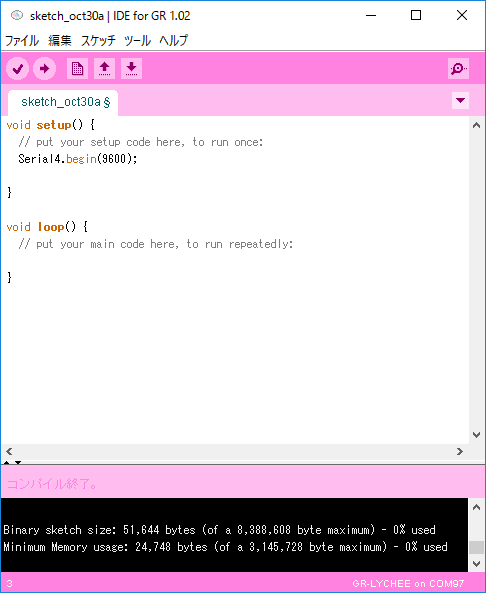
\includegraphics[width=150mm]{ideforgr.png}
 \end{center}
 \caption{IDEforGR}
 \label{fig:idegr}
\end{figure}


\section{モータ制御}
今年度はロボットを3台制作したが,駆動方法は2輪差動と3輪オムニの2種類であり,
特に速さを重視した2輪差動の制御に苦労した.
ロボットを目的地に素早く移動させるために2輪差動を採用したのだが,
操作に用いたDualShock3図\ref{fig:ds3}から得られる数値をそのまま使用した場合,
モータの回転数が最高値に達するのは直進時ではなく旋回時でありコントローラから受け取った数値を補正する必要があった.
また,Arduinoから送っていた制御値がノイズの影響を受けおかしな値になっていたりした.
ロボコンのロボットにおいて駆動部のモータ制御は必要不可欠なため,モータ制御を詳しく説明する.
\begin{figure}[H]
 \begin{center}
  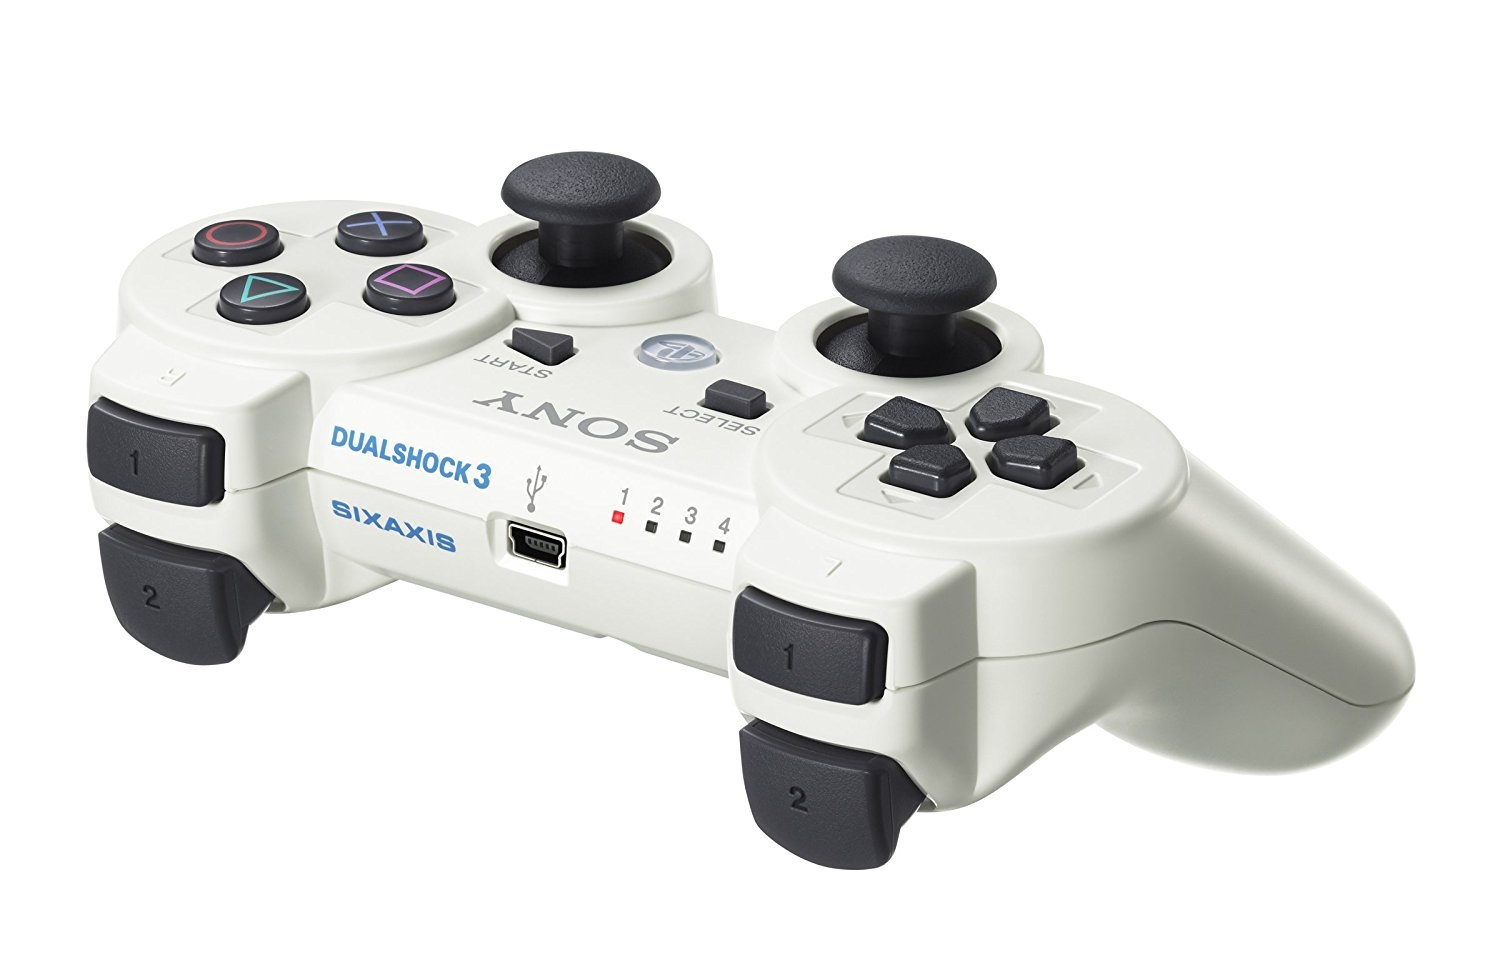
\includegraphics[width=150mm]{dualshock3.jpg}
 \end{center}
 \caption{DualShock3}
 \label{fig:ds3}
\end{figure}
\subsection{2輪差動制御}
今回はDualShock3のアナログスティックを駆動部の操作に用いた.
DualShock3のアナログスティックの可動域は円形をしてるが,数値として出力する値は正方形になっている.
そのため最大の値が出力されるのはスティックをまっすぐ前に倒した時ではなく,斜めに倒した時になる.
今回はロボットの速度を重視した作戦を採用しており,直進時に最高速が出せないのは問題があった.
そこで,コントローラから出力された値にプログラムで正方形からひし形になるように補正をかけた.
補正のイメージ図を図\ref{fig:hosei}に示す.
これにより直進で最高速がでるようになった.
\begin{figure}[H]
 \begin{center}
  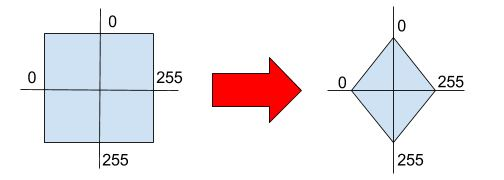
\includegraphics[width=150mm]{hosei.jpg}
 \end{center}
 \caption{補正イメージ}
 \label{fig:hosei}
\end{figure}
実際のプログラムを下に示す.
\begin{lstlisting}[caption=補正Program,label=prg2]
      float d=1.3;
      float x,y;
      int mm;
      
      ly=(float)PS3.getAnalogHat(LeftHatY)-127.5;
      y=ly/127.5;
      
      lx=(float)PS3.getAnalogHat(LeftHatX)-127.5;
      x=lx/127.5;
      
      if (y<=0.0 && 0.0<=x) {     //右上
        w=(y+1.0)*x;
      }
      else if (y<=0.0 && x<=0.0) {//左上
        w=(y+1.0)*x;
      }
      else if (0.0<=y && 0.0<=x) {//右下
        w=-(y-1.0)*x;
      }
      else if (0.0<=y && x<=0.0) {//左下
        w=-(y-1.0)*x;
      }
      else{
        w=0.0;
      }
      
      w=w*500.0;
      w=w*0.8;
      v=y;
      v=v*500.0;
      v=v*0.8;
      
      lm=(int)( (v-(d*w)/2.0) * 0.9 );
      lm=lm+500;
      mm =  motmod( lm , 2 );
      lm=1000-mm;
      //左モータ指令確定
   
      rm=(int)( (v+(d*w)/2.0) * 0.9 );
      rm=rm+500;
      mm = motmod( rm , 1 );
      rm = mm;
      //右モータ指令確定

\end{lstlisting}

\subsection{3輪オムニ制御}
3輪オムニの制御プログラムを下記に示す.
\begin{lstlisting}[caption=補正Program,label=prg2]
Vx = (PS3.getAnalogHat(RightHatX))-127;
      if ((-10<Vx) && (Vx<10)){
        Vy=0;    
      }
      if (Vx < -100) {
        Vx=-100;
      }
      if (Vx >  100){
        Vx= 100;
      }

      Vy = (PS3.getAnalogHat(RightHatY))-127;
      if ((-10<Vy) && (Vy<10)){
        Vy=0;    
      }
      if (Vy < -100) {
        Vy=-100;
      }
      if (Vy >  100) {
        Vy= 100;
      }

      vf = (-1)*Vx;
      vl = (int)(0.5*Vx-0.866*Vy);
      vr = (int)(0.5*Vx+0.866*Vy);

      nvf = (int)(vf*100 / (float)vMAX);
      nvl = (int)(vl*100 / (float)vMAX);
      nvr = (int)(vr*100 / (float)vMAX);

      pwm_f = (int)(nvf*pMAX/100); 
      if(pwm_f>pMAX) {
        pwm_f = pMAX; 
      }
      pwm_l = (int)(nvl*pMAX/100);
      if(pwm_l>pMAX) {
        pwm_l = pMAX;
      }
      pwm_r = (int)(nvr*pMAX/100);
      if(pwm_r>pMAX) {
        pwm_r = pMAX;
      }

      v1=(int)((pwm_f*5.55+999)/2);
      v2=(int)((pwm_l*4.044+999)/2);
      v3=(int)((pwm_r*4.044+999)/2);
      if (right==1){
        v1=v1-mROT;
        v2=v2-mROT;
        v3=v3-mROT;
      }
      if (left==1){
        v1=v1+mROT;
        v2=v2+mROT;
        v3=v3+mROT;
      }
    
      sprintf(m1,"%d%d%d\r\r",v1,v1,v1);
      sprintf(m2,"%d%d%d\r\r",v2,v2,v2);
      sprintf(m3,"%d%d%d\r\r",v3,v3,v3);
\end{lstlisting}

\subsection{ノイズ対策}
今年度のロボット製作で一番悩まされたのはおそらくノイズである.
ノイズとは電気信号の無作為な変動であり,全ての電気回路に存在する.
電子機器が発生するノイズは様々で,その発生原因もいくつもある.
信号線をアルミホイルで巻くなど色々な方法でノイズ対策を行ったが,ここではプログラムに関するノイズ対策を説明する.
プログラム上で行ったノイズ対策はモータドライバに送る3桁の指令値を3回送り多数決で正しい指令値を判定するというものである.

\section{映像ストリーミングシステム}
カタパルトで紙飛行機を発射する際の照準として搭載したカメラ映像をヘッドアップディスプレイに映し出すもの.
システムの概要を図\ref{fig:hud}に示す.
\begin{figure}[H]
 \begin{center}
  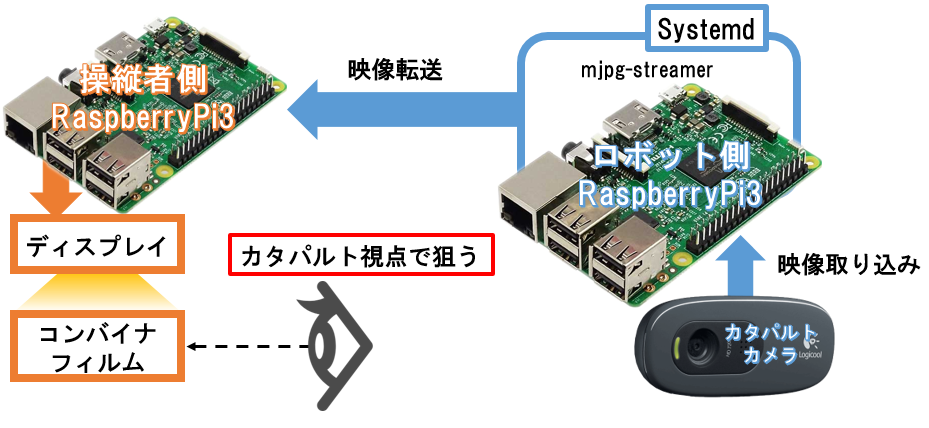
\includegraphics[width=150mm]{hud.png}
 \end{center}
 \caption{映像ストリーミングシステム}
 \label{fig:hud}
\end{figure}

\subsection{映像ストリーミングソフトウエアのインストール}
mjpg-streamerというソフトを使用して映像をストリーミングする.
まず,mjpg-streamerに必要なパッケージであるsubversion、libjpeg-dev、imagemagick、をインストールする.\\
\fbox{sudo apt-get install subversion libjpeg-dev imagemagick}
次に,mjpg-streamerをダウンロードしビルドする.\\
\fbox{svn co https://svn.code.sf.net/p/mjpg-streamer/code/mjpg-streamer mjpg-streamer}\\
\fbox{cd mjpg-streamer}\\
\fbox{make}\\
mjpg-streamerを起動する.
この状態だとネットワーク上に映像をストリーミングしていることになる.\\
webブラウザでRspberryPiのポート8080にアクセスすると映像を確認できる.

\subsection{自動起動}
ロボットに搭載したRaspberryPiを外部から操作するのは困難だったため,
RaspberryPiが起動したと同時に映像ストリーミングが開始されるようにした.
まず,mjpg-streamerを起動するためのListing\ref{shell}シェルスクリプトstream.shを作成する.\\
\fbox{nano stream.sh}\\
\begin{lstlisting}[caption=シェルスクリプト,label=shell]
#!/bin/sh
 
# This is Web-streaming server start up script.for raspi
# No warrantly.
 
# Config
PORT="8081"
ID="ベーシック認証のID" 
PW="ベーシック認証のパスワード" 
SIZE="640x480" 
F_RATE="15" 
MJPG_STREAMER=/usr/local/bin/mjpg_streamer
 
export LD_LIBRARY_PATH=/usr/local/lib
$MJPG_STREAMER \
-i "input_uvc.so -f $F_RATE -r $SIZE -d /dev/video0 -y" \
-o "output_http.so -w /usr/local/www -p $PORT -c $ID:$PW" -b
\end{lstlisting}
ファイルを実行可能なパーミッションに変更するコマンドを実行する.\\
\fbox{chmod 755 stream.sh}\\
次に,systemdを使ってシェルスクリプトを自動起動させるためのserviceファイルstream.serviceを/etc/systemd/systemに作成する.
\begin{lstlisting}[caption=serviceファイル,label=service]
[Unit]
Description = Movie Streaming

[Service]
ExecStart=/home/pi/systemd/stream.sh
Restart=always
Type=simple

[Install]
WantedBy=multi-user.target
\end{lstlisting}
自動起動を有効化するためのコマンドを実行する.\\
\fbox{sudo systemctl enable stream.service}
有効化されたか確認するには,\\
\fbox{sudo systemctl status stream.service}
というコマンドを実行し,enabledと表示されれば有効化されている. 


\subsection{アドホック通信}
mjpg-streamerをそのまま使ってもネットワーク環境がないと映像を見ることができない.
そのため2台のRaspberryPiを1対1でアドホック通信させ,ネットワーク環境がない状況でも映像ストリーミングを可能にさせる.
アドホック通信をするためにRaspberryPiの/etc/network/interfacesをListings\ref{adhoc}のように書き換える.
\begin{lstlisting}[caption=interfaces,label=adhoc]
auto wlan0
iface wlan0 inet static 
address 192.168.12.1 
netmask 255.255.255.0 
wireless-channel 1 
wireless-mode ad-hoc 
wireless-essid pi 
wireless-key 01234567890123456789012345
\end{lstlisting}
受信側も同じようにinterfacesを書き換えるが,addressの下一桁を違う数字に変える必要がある.
wireless-keyは任意の数字でいいが,26桁の16進数である必要がある.
アドホック通信ができているか確認するにはpingコマンドを使用する.\\
\fbox{ping 192.168.12.1}\\
このようにpingのあとに相手のaddressを入れる.

\section{プログラム}

記録したいデータを読み取り,SDカードに書き込むプログラムをListing \ref{prg1}に示す.
\begin{lstlisting}[caption=ログProgram,label=prg1]
#include<Arduino.h>                                             //
#include<SD.h>                                                  //
#include<sdmmc.h>                                               //
#include<data.h>                                                //記録するデータリスト

unsigned long time=0;
int i,j;
float data;


void loging(void){
	file = SD.open("log.txt", FILE_WRITE);      //書き込み用のファイル生成
	
	while(data_seq[i] >= countA){            //記録するデータの種類だけループ
		while(1){
			if(dataB_seq[j] == data_seq[i]){
				check();
				file.print(dataB_seq[j]);            //データの値を書き込み
				break;
			}
			else{ j=j++;
			}
		}
			i=i++;

	}
	file.println(time);                              //タイムスタンプを書き込み改行
}

void setup() {
	File file = SD.open("data.txt", FILE_READ);   //テキストファイルを開く
	while(file.available()){                         //data.txtの中身の数だけループ
		data_seq[i]=file.read();           //記録したいデータの種類がいくつあるか読む
		countA=countA++;                             //記録するデータの種類のカウント
		i=i++;                   
	}	
	time = millis();                                        
}



void loop(){
	loging();                                        //関数呼び出し
}


\end{lstlisting}

各種IOを数字に置き換え,指定されたデータの値を代入するためのヘッダファイル.
\begin{lstlisting}[caption=ヘッダファイル data.h,label=heda]

//データ表
RXD0    = 0 		//PIN_P21
TXD0    = 1 		//PIN_P20
Temp    = 2 		//PIN_P22
Voltage = 3 		//PIN_P23
PIN_P24 = 4		
PIN_P25 = 5 		
PIN_P32 = 6 		
PIN_P33 = 7		
PIN_PC2 = 8		
PIN_PC3 = 9		
PIN_PC4 = 10		
PIN_PC6 = 11		
PIN_PC7 = 12		
PIN_PC5 = 13		
PIN_P40 = 14		
PIN_P41 = 15		
PIN_P42 = 16		
PIN_P43 = 17		
PIN_P44 = 18		
PIN_P45 = 19		
PIN_P46 = 20		
PIN_P47 = 21		
PIN_PC0 = 22		
PIN_PC1 = 23		
PIN_P50 = 24		
PIN_P51 = 25		
PIN_P52 = 26		
PIN_P53 = 27		
PIN_P54 = 28		
PIN_P55 = 29		
PIN_P12 = 30		
PIN_P13 = 31		
PIN_P14 = 32		
PIN_P15 = 33		
PIN_P16 = 34		
PIN_P17 = 35		
PIN_PD0 = 36		
PIN_PD1 = 37		
PIN_PD2 = 38		
PIN_PD3 = 39		
PIN_PD4 = 40		
PIN_PD5 = 41		
PIN_PD6 = 42		
PIN_PD7 = 43		
PIN_PE0 = 44		
PIN_PE1 = 45		
PIN_PE2 = 46		
PIN_PE3 = 47		
PIN_PE4 = 48		
PIN_PE5 = 49		
PIN_PE6 = 50		
PIN_PE7 = 51		
PIN_P07 = 52		
PIN_P05 = 53		
PIN_P35 = 54		
PIN_PJ3 = 55		



//データの値代入
void check(void){
	if(j==0){
		data=PIN_P21               //RXD0
	}
	else if(j==1){
		data=PIN_P20               //TXD0
	}
	else if(j==2){
		data=PIN_P22
	}		
	else if(j==3){
		data=PIN_P23
	}
	else if(j==4){
		data=PIN_P24
	}
	else if(j==5){
		data=PIN_P25
	}
	else if(j==6){
		data=PIN_P32               //TXD6
	}
	else if(j==7){
		data=PIN_P33               //RXD6
	}
	else if(j==8){
		data=PIN_PC2               //SPI_CS3
	}
	else if(j==9){
		data=PIN_PC3
	}
	else if(j==10){
		data=PIN_PC4               //SPI_CS0
	}
	else if(j==11){
		data=PIN_PC6               //SPI_MOSI
	}
	else if(j==12){
		data=PIN_PC7               //SPI_MISO
	}
	else if(j==13){
		data=PIN_PC5               //SPI_CLK
	}
	else if(j==14){
		data=PIN_P40               //dataD0
	}
	else if(j==15){
		data=PIN_P41               //dataD1
	}
	else if(j==16){
		data=PIN_P42               //dataD2
	}
	else if(j==17){
		data=PIN_P43               //dataD3
	}
	else if(j==18){
		data=PIN_P44               //dataD4
	}
	else if(j==19){
		data=PIN_P45               //dataD5
	}
	else if(j==20){
		data=PIN_P46               //dataD6
	}
	else if(j==21){
		data=PIN_P47               //dataD7
	}
	else if(j==22){
		data=PIN_PC0               //SPI_CS1
	}
	else if(j==23){
		data=PIN_PC1               //SPI_SC2
	}
	else if(j==24){
		data=PIN_P50               //TXD2
	}
	else if(j==25){
		data=PIN_P51
	}
	else if(j==26){
		data=PIN_P52               //RXD2
	}
	else if(j==27){
		data=PIN_P53
	}
	else if(j==28){
		data=PIN_P54
	}
	else if(j==29){
		data=PIN_P55
	}
	else if(j==30){
		data=PIN_P12               //IRQ2 / RXD2
	}
	else if(j==31){
		data=PIN_P13               //IRQ3
	}
	else if(j==32){
		data=PIN_P14               //IRQ4 / DPUPE
	}
	else if(j==33){
		data=PIN_P15               //IRQ5 / SDcdatard
	}
	else if(j==34){
		data=PIN_P16               //IRQ6 / VBUS
	}
	else if(j==35){
		data=PIN_P17               //IRQ7
	}
	else if(j==36){
		data=PIN_PD0
	}
	else if(j==37){
		data=PIN_PD1
	}
	else if(j==38){
		data=PIN_PD2
	}
	else if(j==39){
		data=PIN_PD3
	}
	else if(j==40){
		data=PIN_PD4
	}
	else if(j==41){
		data=PIN_PD5
	}
	else if(j==42){
		data=PIN_PD6
	}
	else if(j==43){
		data=PIN_PD7
	}
	else if(j==44){
		data=PIN_PE0
	}
	else if(j==45){
		data=PIN_PE1
	}
	else if(j==46){
		data=PIN_PE2
	}
	else if(j==47){
		data=PIN_PE3
	}
	else if(j==48){
		data=PIN_PE4
	}
	else if(j==49){
		data=PIN_PE5
	}
	else if(j==50){
		data=PIN_PE6
	}
	else if(j==51){
		data=PIN_PE7
	}
	else if(j==52){
		data=PIN_P07
	}
	else if(j==53){
		data=PIN_P05               //DdataI
	}
	else if(j==54){
		data=PIN_P35               //NMI
	}
	else if(j==55){
		data=PIN_PJ3
	}
	else {
		Seridatal.print("Loging Error");
	}
\end{lstlisting}

\section{シールド回路図}
\newpage
\begin{landscape}
\begin{figure}[H]
 \begin{center}
  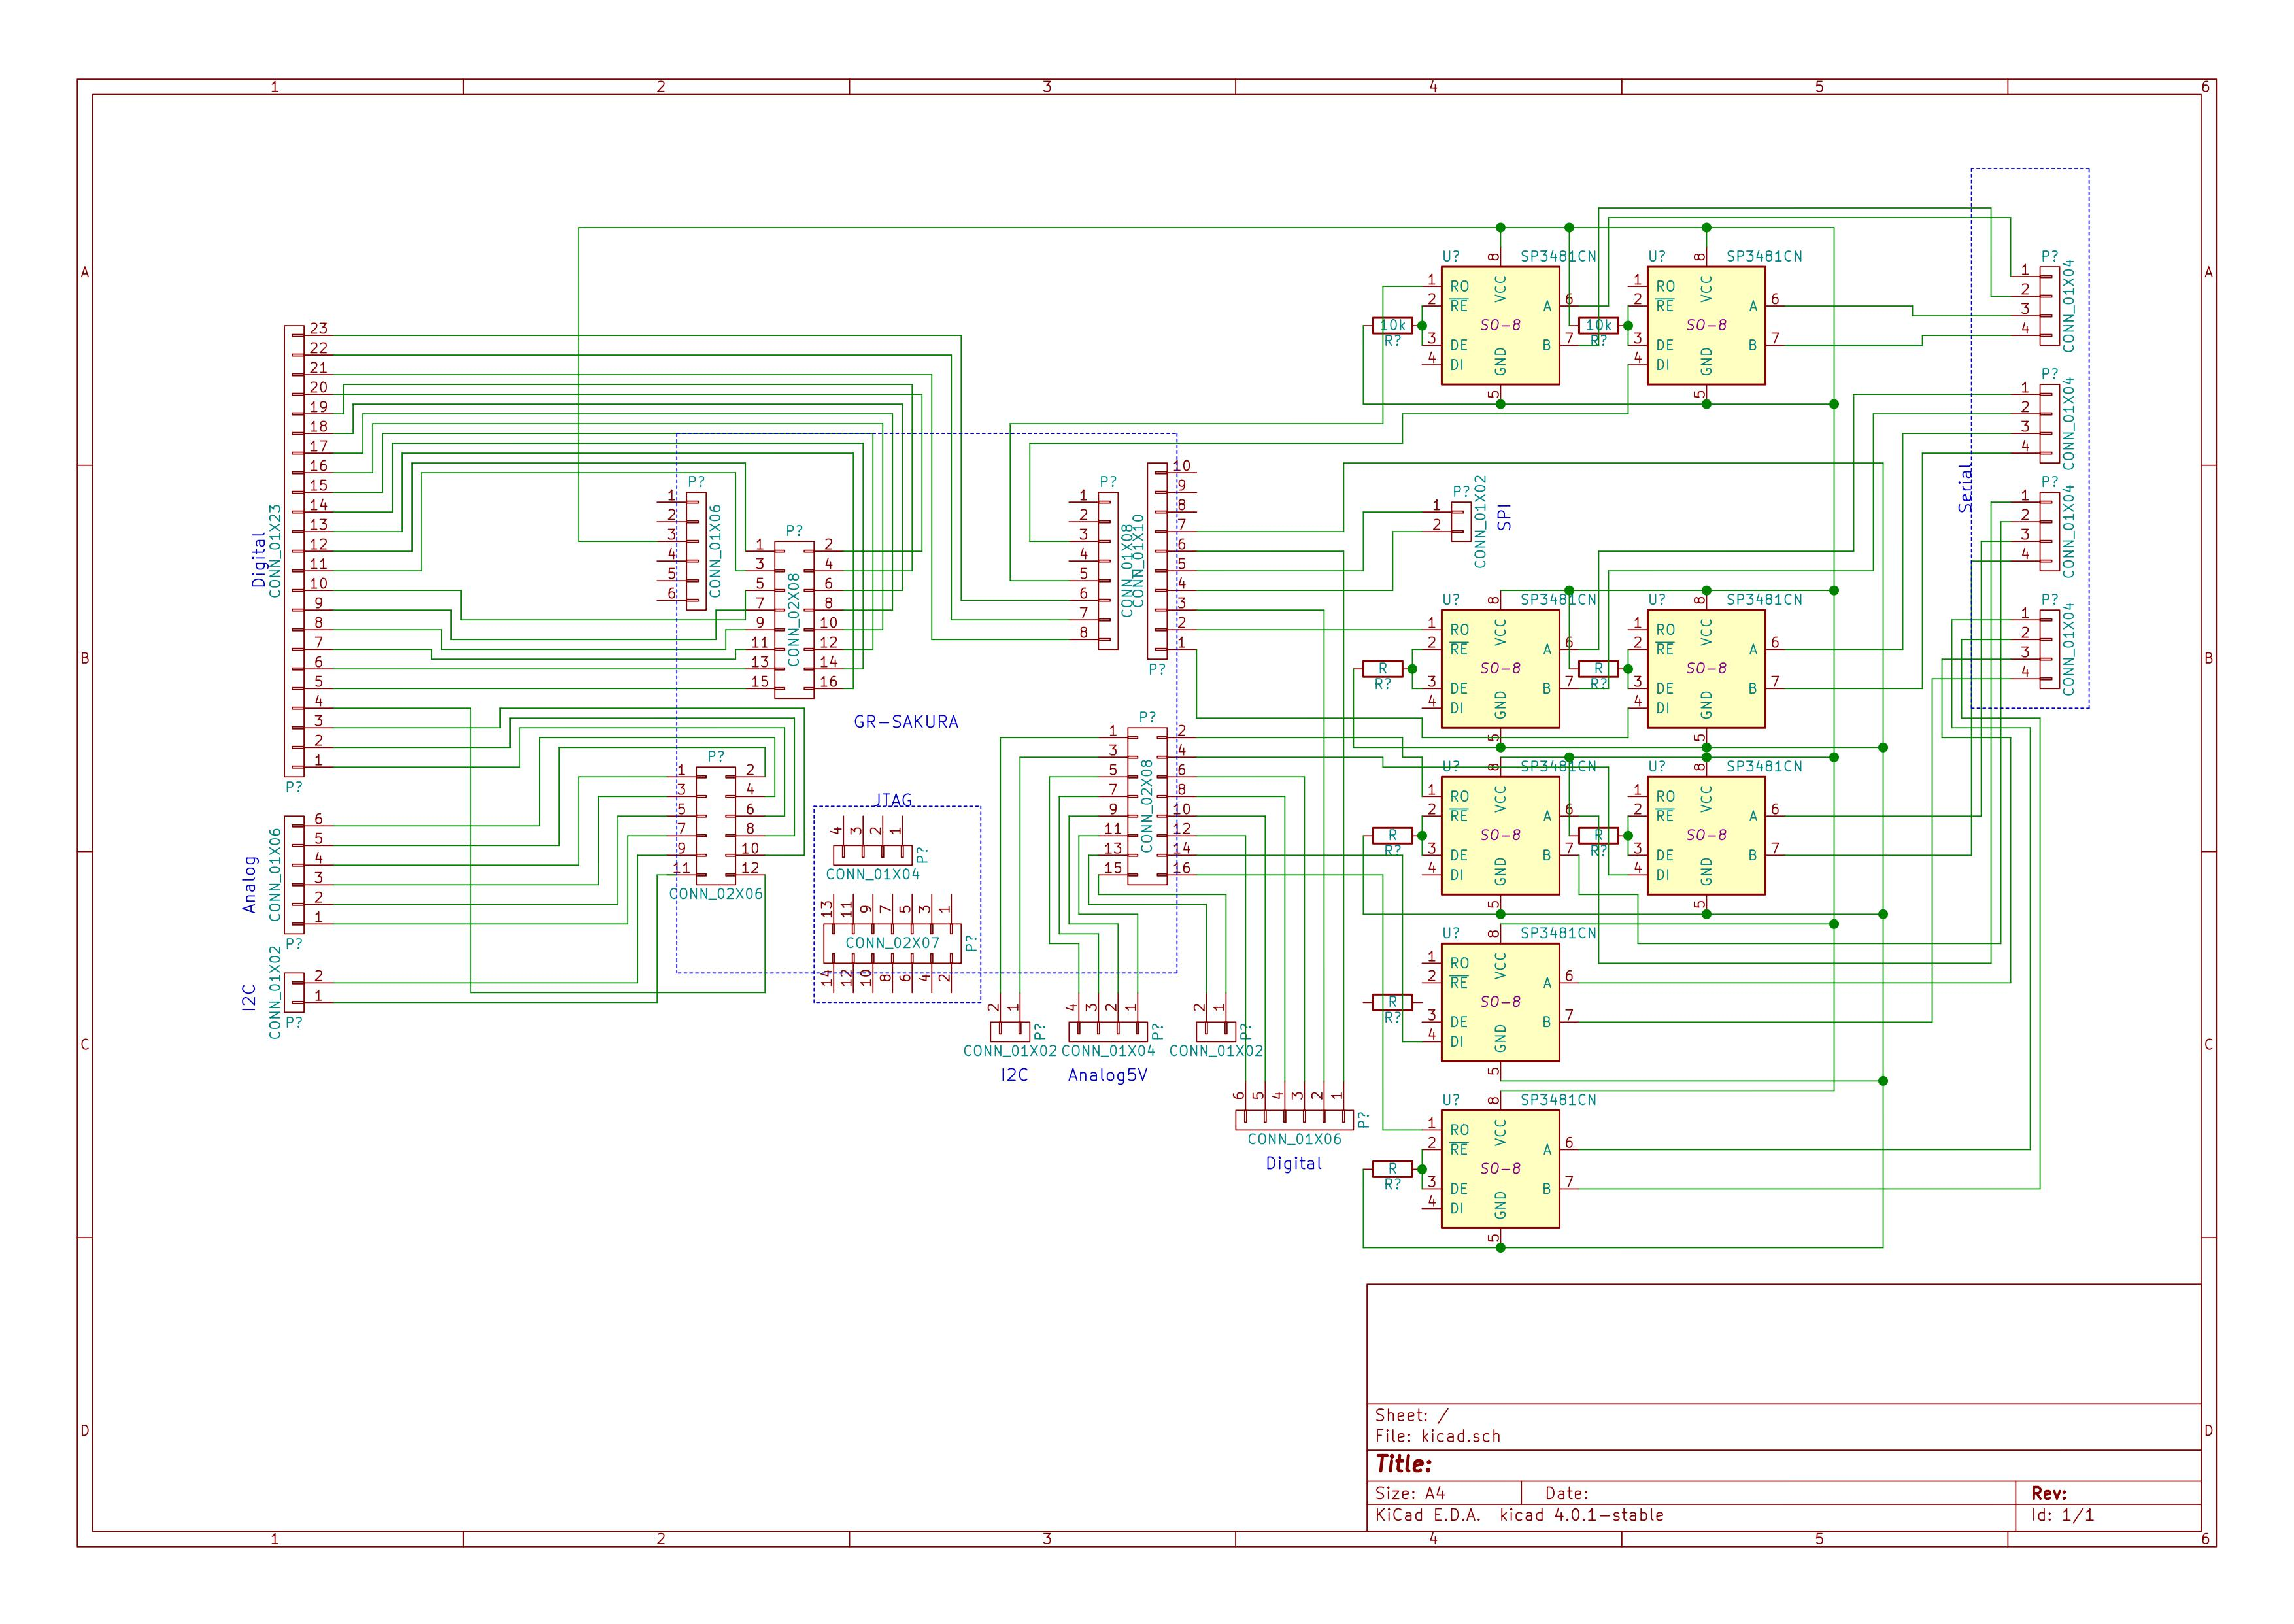
\includegraphics[width=192mm]{0001.jpg}
 \end{center}
 \caption{シールド回路図}
 \label{fig:kairo1}
\end{figure}
\end{landscape}

\end{document}
htpb
